% This is samplepaper.tex, a sample chapter demonstrating the
% LLNCS macro package for Springer Computer Science proceedings;
% Version 2.20 of 2017/10/04
%

\documentclass[runningheads]{llncs}

\usepackage{times}
\usepackage{ifpdf}
\usepackage[english]{babel}
\usepackage{cite}
\usepackage[utf8]{inputenc}

\usepackage{graphicx}
\usepackage{amssymb,amsmath,amsfonts} 
\usepackage{balance}

\usepackage{color}
\usepackage{hyperref}
\usepackage[nocenter]{qtree}
\usepackage{tree-dvips}
\usepackage{listings}

\definecolor{lightgrey}{rgb}{0.97,0.97,0.97}

\newcommand{\IS}		{INScore}
\newcommand{\exemple}	{\vspace*{1mm}\hspace*{-4mm}\textbf{Example :}}

\newcommand{\code}	[2][0.9]	{\vspace{0mm}\begin{center}\colorbox{lightgrey}{
							\begin{minipage}[t]{#1\columnwidth} 
							{\small \texttt{#2}}
							\end{minipage}}\end{center}}

\newcommand{\llist}	[1]		{\ensuremath{[#1_1,...,#1_k]}}

\newcommand{\seq}		{\ensuremath{|}}
\newcommand{\paral}		{\ensuremath{\parallel}}
\newcommand{\forest}	{\ensuremath{\varnothing}}
\newcommand{\toType}	{\ensuremath{\mathcal{T}}}
\newcommand{\toAddress}	{\ensuremath{\text{@}}}
\newcommand{\toOSCAddress}	{\ensuremath{\texttt{OSC}}}
\newcommand{\taddress}	{\ensuremath{\text{@}}}
\newcommand{\toData}	{\ensuremath{\text{D}}}
\newcommand{\tdata}	    {\ensuremath{\text{D}}}
\newcommand{\binop}		{\ensuremath{\texttt{op}}}
\newcommand{\etc}		{\ensuremath{\text{…}}}
\newcommand{\emptyf}	{\ensuremath{[\ ]}}

\newcommand{\nexpand}	{\ensuremath{\varepsilon}}
\newcommand{\ula}		{\hspace*{8mm}}
\newcommand{\ulb}		{\hspace*{31.5mm}}


% ====================================================
\hypersetup{
    colorlinks,%
    citecolor=black,%
    filecolor=black,%
    linkcolor=black,%
    urlcolor=black
}


% ====================================================
\begin{document}

\title{A Tree Based Language for Music Score Description.}

\author{D. Fober\inst{1} \and
Y. Orlarey\inst{1} \and
S. Letz\inst{1} \and R. Michon\inst{1}}
%
\authorrunning{Fober et al.}
% First names are abbreviated in the running head.
% If there are more than two authors, 'et al.' is used.
%
\institute{Grame CNCM  Lyon - France \\ 
\email{{\small \{fober,orlarey,letz,michon\}@grame.fr}}}


\maketitle

%
\begin{abstract}
The presented work is part of the \IS\ project, an environment for the design of augmented interactive music scores, oriented towards unconventional uses of music notation and representation, including real-time symbolic notation capabilities. This environment is fully controllable using Open Sound Control [OSC] messages. \IS\ scripting language is an extended textual version of OSC messages that allows you to design scores in a modular and incremental way. This article presents a major revision of this language, based on the description and manipulation of trees.

\keywords{Music notation \and Language \and INScore.}
\end{abstract}
%

%-------------------------------------------------
\section{Introduction}\label{sec:introduction}

There is a large number of musical score description languages (Lilypond \cite{lilypond03}, Guido \cite{hoos98}, MuseData \cite{Hewlett97}, MEI \cite{Roland_2002}, MusicXML \cite{good01} etc.) that are all turned towards common western music notation. 
The extension of some of these languages has been considered, in order to add \textit{programmability} e.g. operations to compose musical scores in Guido \cite{fober12b}, or the Scheme language in Lilypond.
There are also programming languages dedicated to common music notation, like CMN \cite{Schottstaedt97} or ENP 
\cite{KUUSK06} that are actually Lisp dialects. %, always oriented towards the common western notation.

The approach proposed by \IS\ \cite{Fober:12a} is different: symbolic music notation is supported (via the Guido language and rendering engine \cite{Dau:09b,hoos98}), but it constitutes one of the means of music representation among others, without being privileged. 
Purely graphic scores can be designed. All the elements of a score (including purely graphical elements) have a temporal dimension (date, duration and tempo) and can be manipulated both in the graphic and time space. The notion of time is both event-driven and continuous \cite{fober17c}, which makes it possible to design interactive and dynamic scores. Figure \ref{pavlos} presents an example of a score realised using \IS . It includes symbolic notation, pictures, a video, and cursors (the video is one of them) which positions are synchronised by the performer gestures.

\begin{figure}
\begin{center}
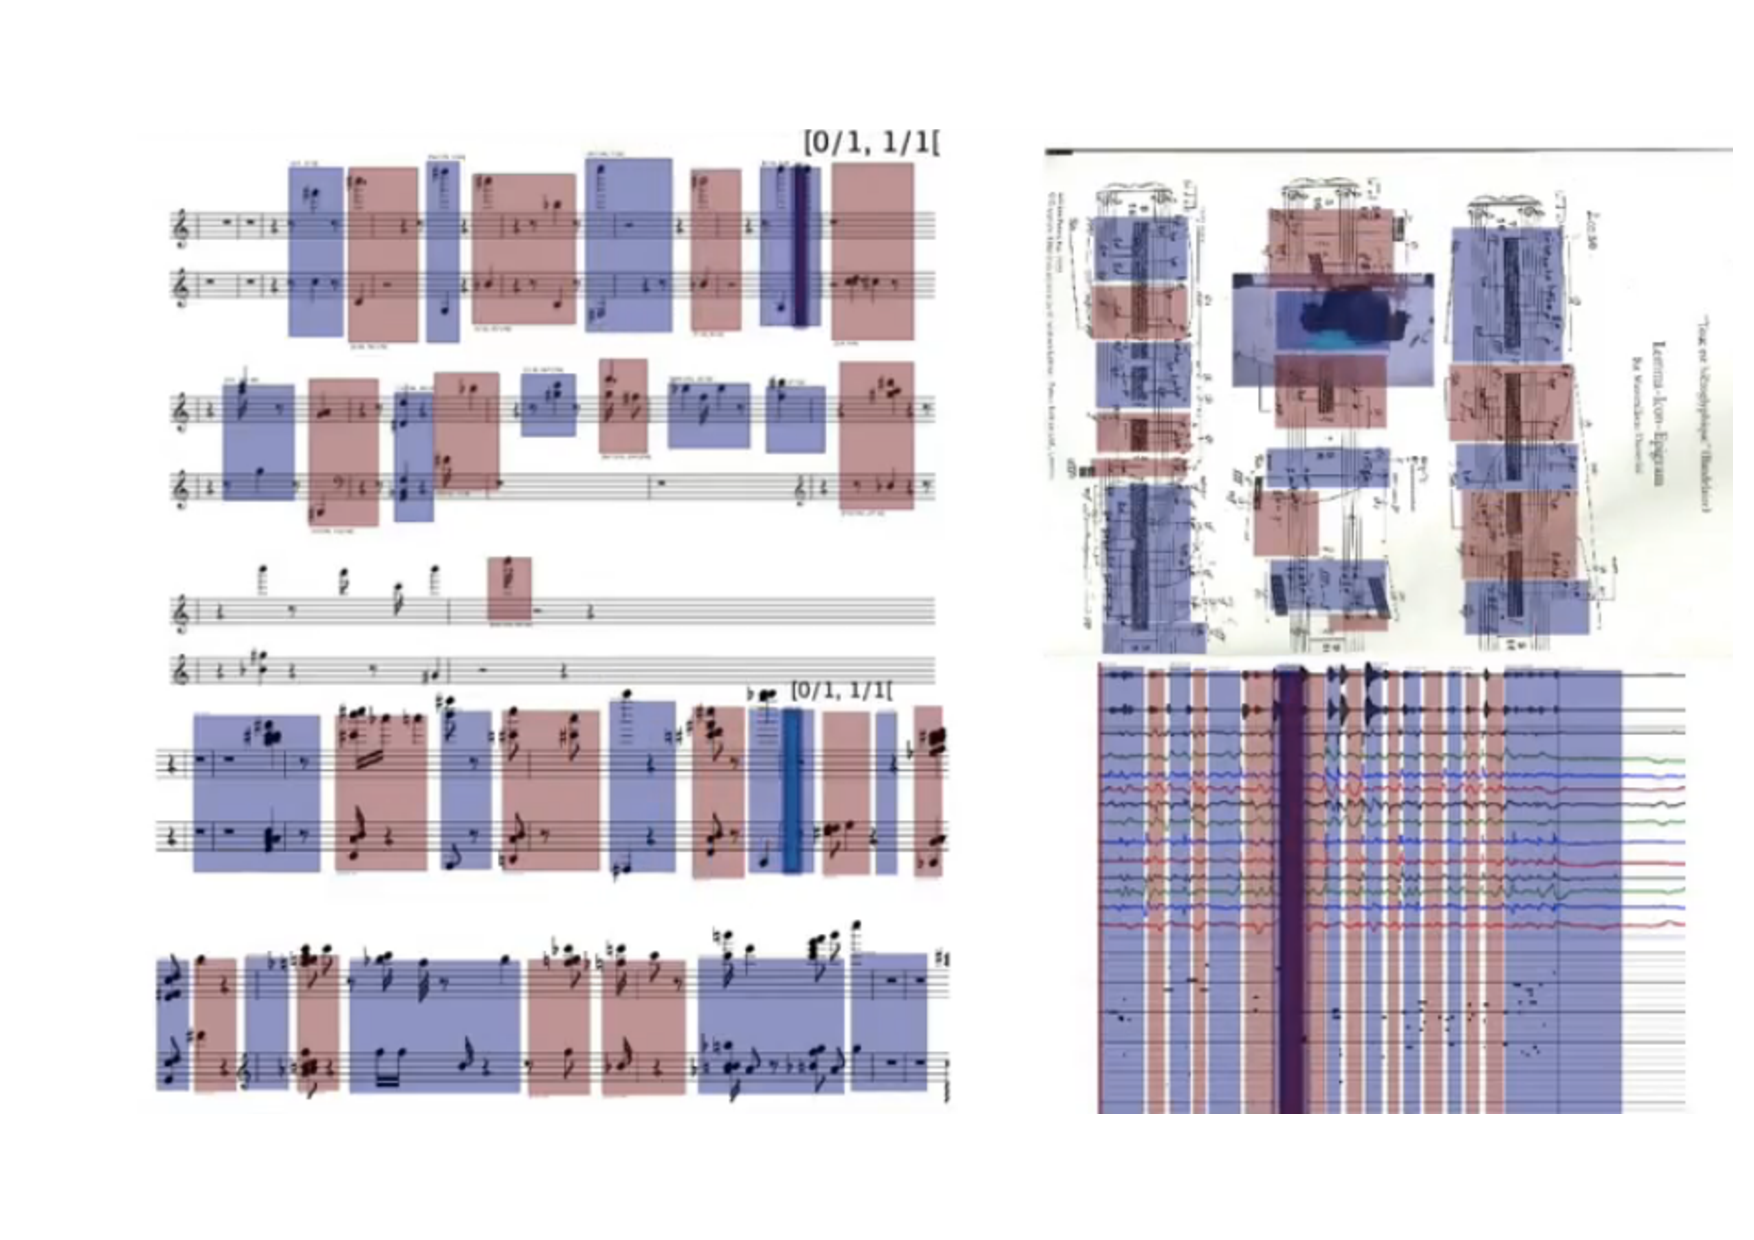
\includegraphics[width=0.64\columnwidth]{imgs/inscore-score}
\caption{A score realised using \IS , used as part of a sensor-based environment for the processing of complex music called \emph{GesTCom} (\emph{Gesture Cutting through Textual Complexity}) \cite{antoniadis:tel-01861171}.}
\label{pavlos}
\end{center}
\end{figure}

\IS\ has been initially designed to be driven by OSC messages \cite{OSC}. OSC is basically a communication protocol. A textual version of the OSC messages constitutes the \IS\ storage format, which has been extended to a scripting language, \cite{Fober:13b} allowing greater flexibility in music scores design.
These extensions (variables, extended addresses, Javascript section, etc.) have nevertheless suffered from a rigidity inherent to an ad hoc and incremental design. For example, the parser makes a clear distinction between OSC addresses and associated data, which prevents the use of variables in OSC addresses.
Thus, a major revision of this language became necessary. It is based on the manipulation of a regular tree structure that is also homogeneous to the \IS\ model.
Figure \ref{tree1} gives an example of such model hierarchy, that can be described in the current scripting language (i.e. OSC) by listing all branches from the root. % (Figure~\ref{script1})

\begin{figure}
\begin{center}
\Tree [ .ITL [ .scene 
	[ .obj1 [ .x 0 ] [ .y 0 ] [ .date 0 ] ] 
	[ .obj2 [ .x 0.5 ] [ .y 0.5 ] [ .date 1 ] ] ] 
]
\caption{A score sample including 2 objects $obj1$ and $obj2$, having $x$, $y$, and $date$ attributes. Time properties (date, duration) are notably used to represent the time relationship between objects.}
\label{tree1}
\end{center}
\end{figure}

After some definitions, we will present the basic operations on trees and the corresponding grammar.Then we introduce mathematical operations on trees, the concepts of \emph{variables} and \emph{nodes in intention} and we'll present how this language is turned into OSC messages. The final section gives an example of the new language before concluding.


%-------------------------------------------------
\section{Definitions}

A tree $t$ consists of a value $v$ (of some data type) and the (possibly empty) list of its subtrees.
\[
	t :  v \times\llist{t} 
\]
A tree with an empty list of subtrees $t:v\times \emptyf$ is called a leaf.\\
A value is among literal (i.e., text, number) or special values of the following types:
\begin{itemize}
\item forest (\forest): denotes a tree including only subtrees,
\item mathematical operators: indicates a mathematical operation between subtrees,
\item variable: denotes a tree whose value refers to another tree, 
\item expand: indicates a tree to be expanded,
\item slash (/): used for conversion to OSC
\end{itemize}
Use and evaluation of these values is detailed in the next sections.

%-------------------------------------------------
\section{Operations on Trees}

We define two abstract operations on trees: sequencing and paralleling. These operations have no musical semantics, neither from a temporal nor from a graphic point of view. They are defined as methods for algorithmic construction of OSC messages and operate on the topological organisation of the trees. 

%-----------------------------
\subsection{Putting Trees in Sequence}
Putting two trees $t$ and $t'$ in sequence adds $t'$ as child of all the leaves of $t$.
We will note \seq\ the sequencing operation.
Let 2 trees $t :  v \times \llist{t}$ and $t'$.
Then:
\[
	v \times \llist{t} \seq\ t'  \to  v  \times [t_1 \seq\ t',\etc, t_k \seq\ t']
\]
with: 
\[
\left\{
\begin{array}{l}
	v \times \emptyf \seq\ t'  \to  v  \times [ t' ]\\
	v \times \emptyf \seq\ \forest \times \llist{t}  \to  v  \times \llist{t}\\
\end{array}
\right.
\]
The right arrow ($\to$) indicates the result of an expression evaluation.

%-----------------------------
\subsection{Putting Trees in Parallel}
Putting two trees $t$ and $t'$ in parallel consists in putting them in a forest.
We will note \paral\ the parallelisation operation. 
Let 2 trees $t$ and $t'$:
\[
	t \paral\ t'  \to  \forest \times [ t, t' ]
\]
The result is a tree which value \forest\ denotes a forest. \\
Parallelisation applied to a \emph{forest} preserves the subtrees order:
\[
\left\{
\begin{array}{l}
	\forest \times \llist{t}\  \paral\ t'  \to  \forest \times [t_1,\etc,t_k,t']\\
	t' \paral\ \forest \times \llist{t}\   \to  \forest \times [t',t_1,\etc,t_k]\\
\end{array}
\right.
\]


%-------------------------------------------------
\section{Grammar}\label{agram}

A tree is syntactically defined in BNF as follows:
\code{tree := value      \hspace*{8mm} $\to$ t : value \emptyf \\
\ula | tree tree         \hspace*{4mm} $\to$ t : tree \seq\ tree \\
\ula | / tree            \hspace*{9.7mm} $\to$ t : '/' \seq\ tree\\
\ula | tree , tree       \hspace*{0mm}  $\to$ t : tree \paral\ tree \\
\ula | ( tree )          \hspace*{6mm} $\to$ t : tree \\
\ula ;
}
The right arrow ($\to$) indicates the tree built for each syntactical construct. 
The tree whose value is \emph{slash} (/) plays a special role in the tree conversion to OSC messages. This role is described in section \ref{sslash}.


%-------------------------------------------------
\section{Values and Evaluation}\label{sec:valeurs}

This section explains how the trees carrying the special \emph{mathematical operators}, \emph{variables} and \emph{expand} special values are evaluated.

%---------------------------
\subsection{Mathematical Operators}

Mathematical operations on trees are seen as operations on their values that preserve the subtrees. These operations include arithmetic and logical operations, trigonometric and hyperbolic functions, exponential and logarithmic functions, power, square root, etc.

We will designate these operations by \binop. Then for 2 trees $t : v \times \llist{t}$ and $t' : v' \times \llist{t'}$:
\[
	\binop \times [ t, t']  \to  (\binop\ v\ v') \times [ t_1,\etc,t_k,t'_1,\etc,t'_k ]
\]

%---------------------------
\subsection{Variables}
The special value type \emph{variable} denotes a tree whose value refers to another tree.
%A variable is the association of an identifier and a tree. Its general form is
%$varname = t$.
Evaluation of a variable tree consists in expanding the referred tree at the variable position.
Let's define a variable $var$ and a variable tree $t'$ as follows:
\[
\left\{
\begin{array}{l}
	var = v \times \llist{t} \\
	t' : \$var \times \llist{t'}\\
\end{array}
\right.
\]
then 
\[
	t'_{\{var\}}  \to v \times \llist{t}\ \seq\ \forest \times \llist{t'}
\]
t'$_{\{var\}}$ denotes the tree $t'$ with an environment containing a definition of the variable $var$.

\exemple
\code{x = x 0;\\
y = y 0;\\
/A/B \$x, \$y; \ \ $\Rightarrow$  /A/B (x 0), (y 1);}


%---------------------------
\subsubsection{Local Environnements}

Each tree is evaluated in an environment containing the list of all the variables of its parent. However, a variable can be evaluated in a local environment, which is defined inside braces:
\[
\left\{
\begin{array}{l}
	var = t \\
	\$var\{a=t1, b=t2,\etc\} \ \to  t_{\{a, b,\etc\}} \\
\end{array}
\right.
\]


%---------------------------
\subsection{Expand Value}

An \emph{expand value} is a special value that is expanded to a forest. It can also be seen as a \emph{loop} control structure. The syntactic form is as follows:
\begin{description}
\item $id[n\etc m]$ 	where $n$ and $m$ are integers
\item $id[ab\etc xy]$ where $a,b,x,y$ are letters.
\end{description}
We will note \nexpand\ the expansion operation:
\[
\left\{
\begin{array}{l}
	\nexpand(id[n\etc m])   \ \ \to \forest \ [id_n,id_{n+1},\etc ,id_m] \\
	\nexpand(id[ab\etc xy]) \to \forest \ [id_{ab},id_{ac},\etc ,id_{ay}, \\
	\ulb \etc ,\\
	\ulb id_{xb},id_{xc},\etc ,id_{xy}]
\end{array}
\right.
\]
where each $id_n$ is a tree $v \times \emptyf$ whose value $v$ is the concatenation of the base value $id$ and of the current index $n$.

%---------------------------
\subsubsection{Special Forms}

An \emph{expand value} can also take the following special forms: 
\begin{description}
\item $id[i:n\etc m]$ 	where $i$ is an identifier
\item $id[i:j:ab\etc xy]$ where $i,j$ are identifiers.
\end{description}
The identifiers denote variables that are instantiated in the environment by the expansion operation, with the current index value. For example:
\[
	\nexpand(id[i:n\etc m])   \quad \to \forest \ [id_{n\{i=0\}},id_{n+1\{i=1\}},\etc ,id_{m\{i=m-n\}}] \\
\]

%-------------------------------------------------
\section{Conversion to OSC}\label{sslash}

An OSC message is made of an OSC address (similar to an Unix path) followed by a list of data (which can possibly be empty)
The \emph{slash} special value of a tree is used to discriminate the OSC address and the data. \\
We define two types of values: 
\begin{description}
\item \taddress : the type of a value part of an OSC address
\item \tdata : the type of a value part of the OSC data
\end{description}
We'll note $type(v)$ to refer to the type of the value $v$.
Note that in INScore, an OSC message can be part of the OSC data. Thus a value can carry both the \taddress\  and \tdata\ types.
We'll note $t^a$ a tree $t$ which value is of type \taddress\ and $t^d$ a tree $t$ which value is of type \tdata .
Then we define two operations: \toAddress\ and \toData\ that transforms a tree in to a \emph{typed} tree:
\[
    \toAddress (v \times \llist{t}) \to 
\left\{
\begin{array}{l}
	\forest \times \llist{t^a} , v = /\\
	v \ \times \llist{t^d} , v \neq / \\
\end{array}
\right.
\]
\[
    \toData (v \times \llist{t}) \to v \ \times \llist{t^d} , type(v) = D
\]
%The \toData\ operation actually propagate the \tdata\ type to all the children of the first tree of type \tdata .

The conversion of a tree $t$ into OSC messages transforms the typed tree $\toData (\toAddress (t))$ into a forest of OSC addresses followed by data.
\[
    \toOSCAddress (v \times \llist{t}) \to
\left\{
\begin{array}{l}
	\forest \times [ v \times \toOSCAddress(t_1),\etc , v \times \toOSCAddress(t_k)] , type(v) = \taddress\\
	v \ \times \llist{t} , type(v) = \tdata \\
\end{array}
\right.
\]


% \[
% \left\{
% \begin{array}{l}
% 	\toType (/ \times \llist{t}) \to \forest \times \llist{t^a} \\
% 	\toType (v \times \llist{t}) \to v \times \llist{t^d} \ \land v \neq / \lor \\
% \end{array}
% \right.
% \]


% Transforming a tree into a list of OSC messages consists in transforming this tree into a forest of \emph{osc trees}. An \emph{osc tree} is a tree made of an OSC address followed by data:
% \[
% 	OSC : osc\_address \times \llist{d}
% \]

% Transforming a tree into OSC messages consists in enumerating all the paths from the root node up to the first parameter, which is the first node that is not preceded by a \emph{slash}.



%-------------------------------------------------
\section{Example}\label{example}

The script below presents an example of the new version of the \IS\ scripting language. Variables are indicated in blue. Local variables are declared in red.

\lstdefinelanguage{inscore} 
{
classoffset=0,
morekeywords={}, keywordstyle=\color{blue},
classoffset=1,
morekeywords={addr, count, radius, size, pos, color }, keywordstyle=\color{red},
classoffset=2,
keywordsprefix=$,
sensitive=true,
morecomment=[l]{\#},
morestring=[b]", 
}

\lstset{backgroundcolor=\color{lightgrey}, extendedchars=true, inputencoding=utf8}

\begin{lstlisting}[language=inscore, extendedchars=true, basicstyle=\small\ttfamily]
# variables declaration 
pi    = 3.141592653589793;

# '$step' makes use of 'count' a local variable 
step  = / ( * 2, $pi), $count;

# '$i' is defined by the expansion of the address 'n_[i:1...9]'
x = math.sin ( * $step, $i );
y = math.cos ( * $step, $i );

# the following variables select part of guido
# music notation code to build a short score
dyn = (? (% $i, 3), '\i<"p">', '\i<"ff">');
note = (+ $dyn, " ", (?  (% $i, 2), "e2", "g1/8"));

# this is a classical OSC message that simply clears the scene
/ITL/scene/* del;

# this is the main variable. It will be expanded to create 
# a series of small scores. The variables are computed 
# using locally defined variables.  
notes = (/ITL/scene/$addr  
	(set gmn (+ "[", $note, "]")),
	(scale 0.7),
	(x * $x, $radius),
	(y * $y, $radius)); 

# finally '$notes' is used  with addr, count and radius as local
# variables, which could be viewed as a function call.
$notes{addr=n_[i:1...9], count=9, radius=0.7};
\end{lstlisting}


Evaluation of this script produces OSC messages fully compatible with the previous version of the language, and which are schematically presented below. 
\code[1]{/ITL/scene/n\_1 set gmn '[ \i<"ff"> g1/8]';\\
/ITL/scene/n\_1 scale 0.7;\\
/ITL/scene/n\_1 x 0.0;\\
/ITL/scene/n\_1 y 0.7;\\
...\\
/ITL/scene/n\_9 set gmn '[ \i<"ff"> c2]';\\
/ITL/scene/n\_9 scale 0.7;\\
/ITL/scene/n\_9 x -0.411452;\\
/ITL/scene/n\_9 y 0.56631;
}
In practice, this example expresses the score illustrated in Figure \ref{samplescene} in just a few lines.  

\begin{figure}[htbp]
\begin{center}
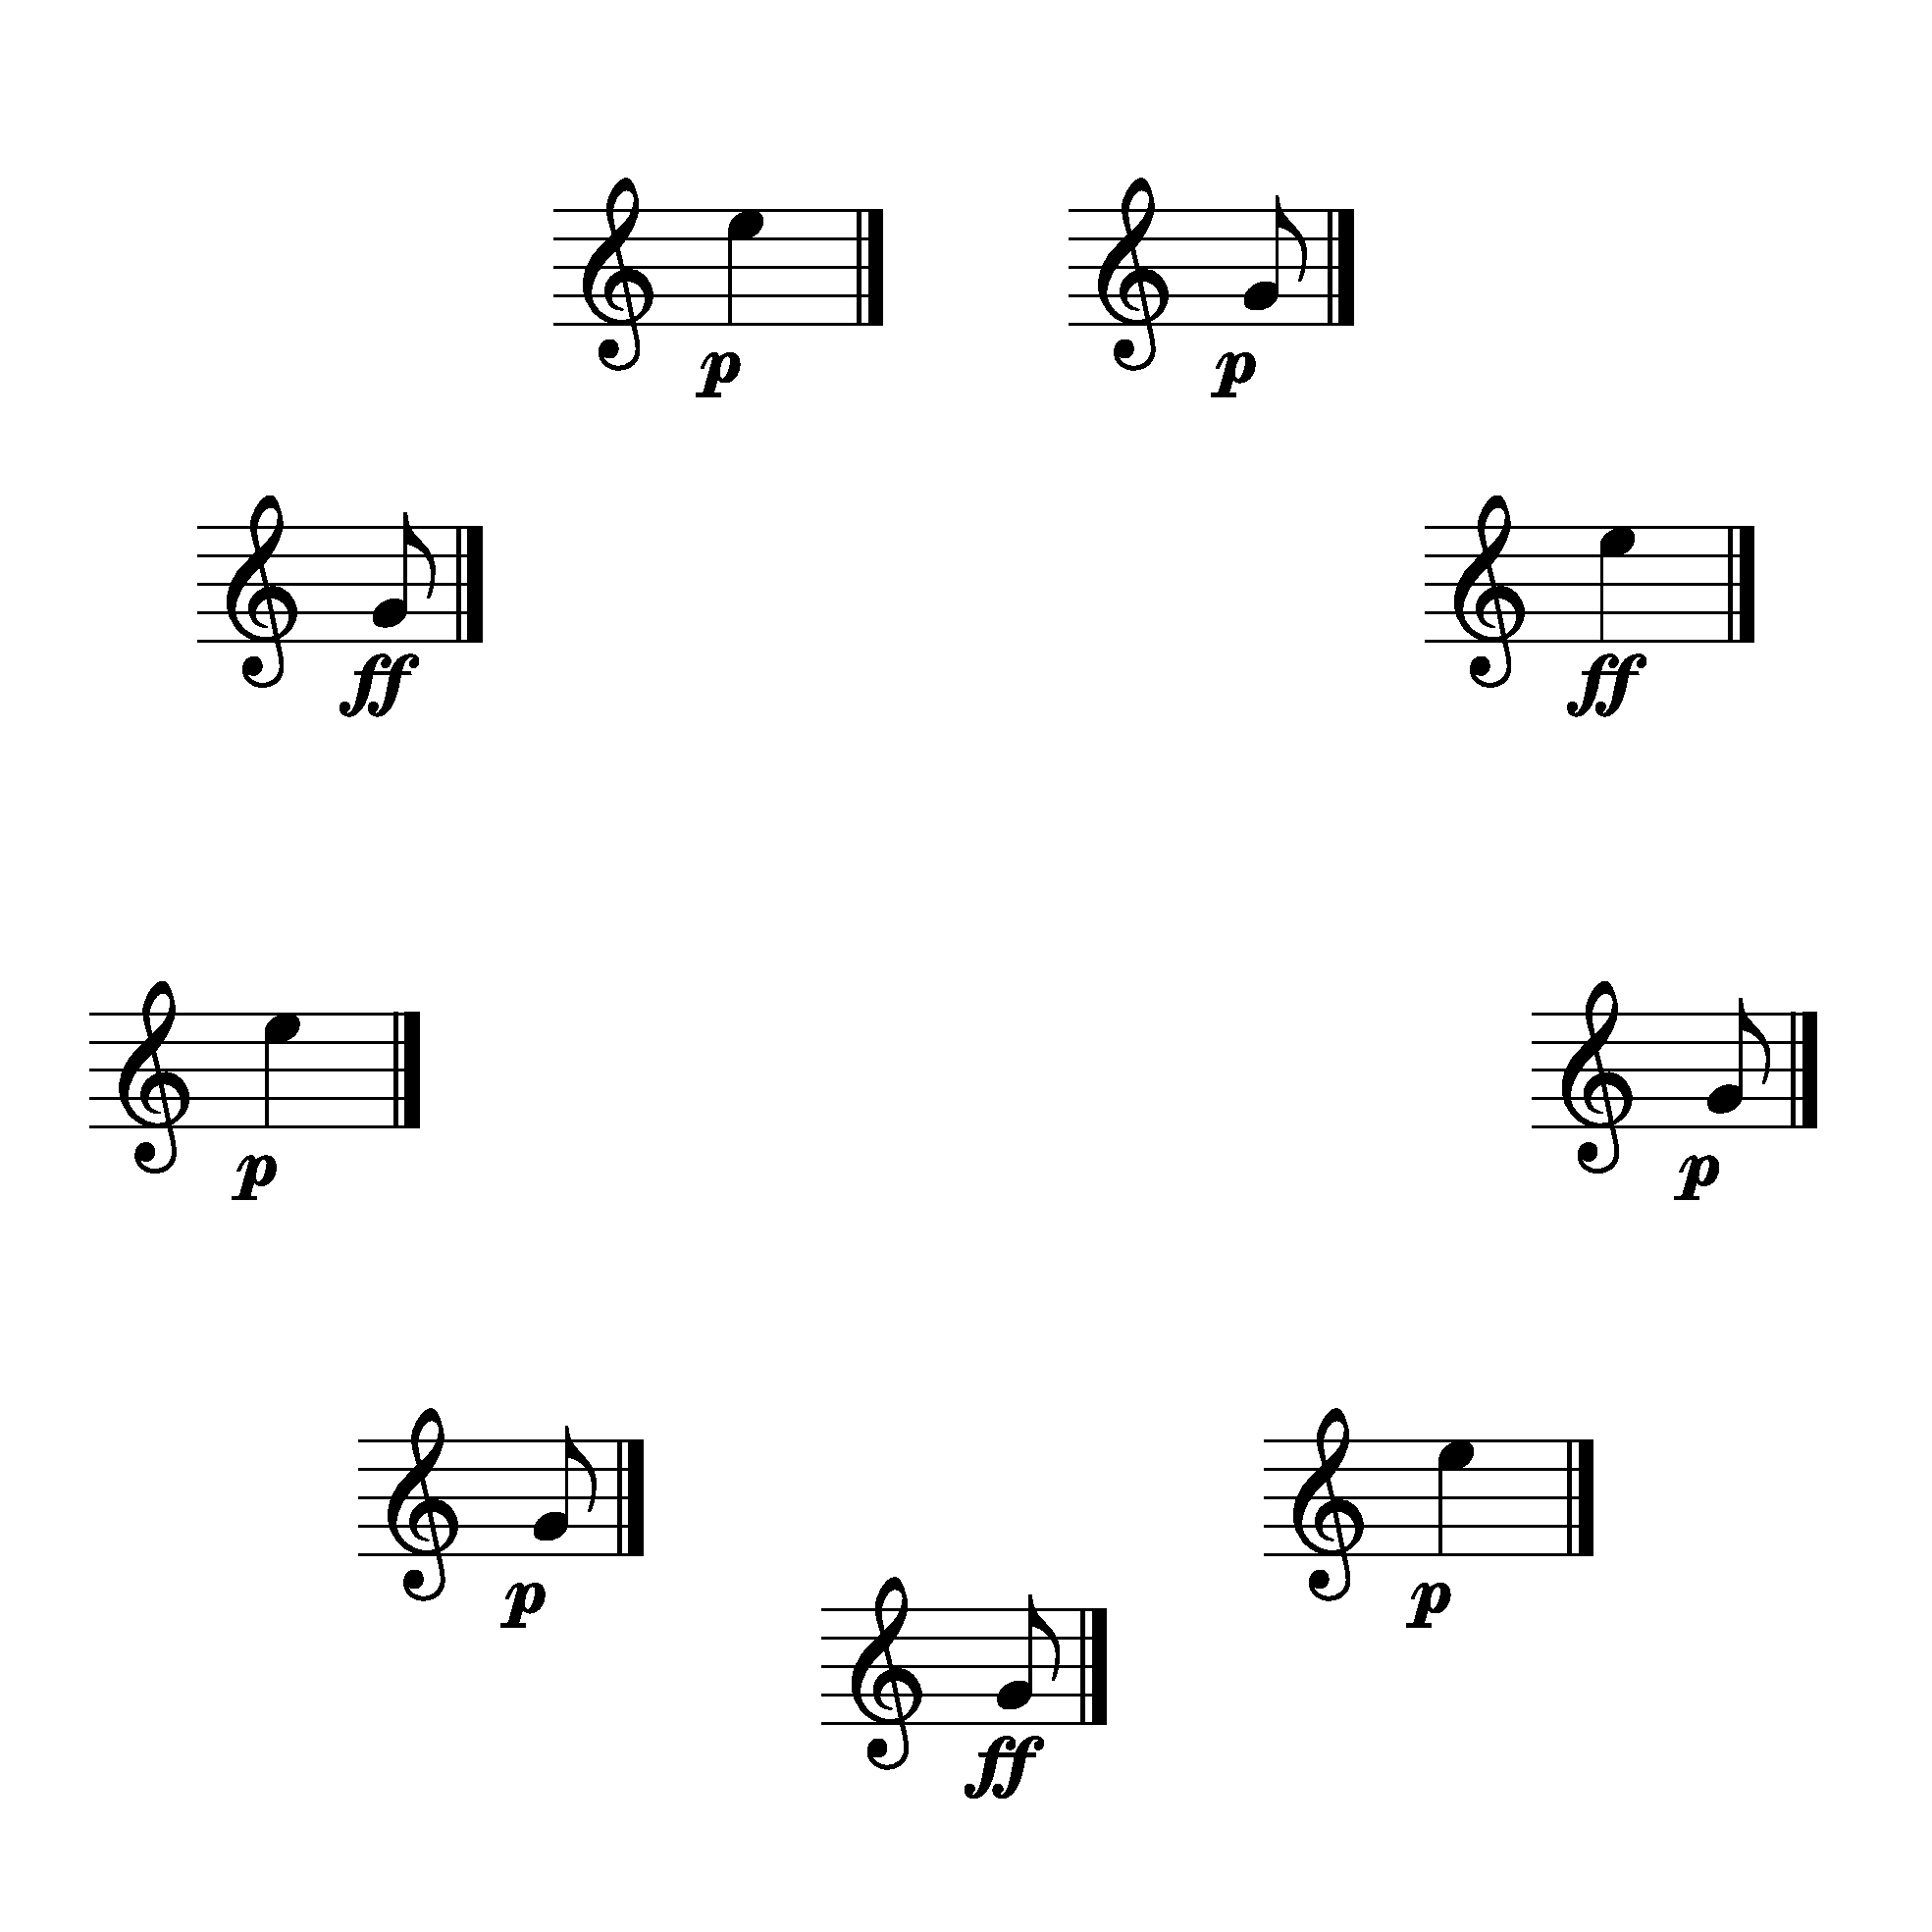
\includegraphics[width=0.8\columnwidth]{imgs/scene}
\caption{\IS\ scene corresponding to the sample script given in section \ref{example}.}
\label{samplescene}
\end{center}
\end{figure}


%-------------------------------------------------
\section{Conclusions}
From two elementary operations on trees - sequencing and parallelisation - we have homogeneously introduced the notions of variables and of mathematical and logical operations on trees. The resulting language is much more expressive and more flexible than the  previous version of the \IS\ scripting language. 
It supports parallelisation of the arguments of a message, variables to describe addresses, series of addresses expressed in a concise manner, use of local variables allowing reusing scripts or parts of scripts in different contexts.



%%%%%%%%%%%%%%%%%%%%%%%%%%%%%%%%%%%%%%%%%%%%%%%%%%%%%%%%%%%%%%%%%%%%%%%%%%%%%
%bibliography here
\balance
\bibliographystyle{splncs04}
\bibliography{../interlude}

\end{document}
